\clearpage

\subsection{Transparent without Survivability}\label{heuristic_Transp_Survivability}
\begin{tcolorbox}	
\begin{tabular}{p{2.75cm} p{0.2cm} p{10.5cm}} 	
\textbf{Student Name}  &:& Pedro Coelho    (01/03/2018 - )\\
\textbf{Goal}          &:& Implement the heuristic model for the transparent transport mode without survivability.
\end{tabular}
\end{tcolorbox}

\vspace{11pt}
In the transparent transport mode (single-hop approach), the signals travel through the network in the optical domain between lightpaths. One advantage of this transport mode is that these networks require optical switching. This enables the realization of ongoing optical connections throughout several links without OEO (optical-electrical-optical) conversions. However, there are performed some conversions in some intermediate nodes.

Transparent optical connections creates lightpaths which require the assignment of a wavelength that will be used to be exchanged by wavelength converters in order to optimize the network and minimize the total CAPEX.

After the creation of the matrices and the network topology, it is necessary to apply the routing and grooming algorithms created. In the end, a report algorithm will be applied to obtain the best CAPEX result for the network in question.

We also must take into account the following particularity of this mode of transport:
\begin{itemize}
  \item $N_{OXC,n}$ = 1, \quad $\forall$ n that process traffic
  \item $N_{EXC,n}$ = 1, \quad $\forall$ n that process traffic
\end{itemize}

The minimization of the network CAPEX is made through the equation \ref{Capex_heuristic} where in this case for the cost of nodes we have in consideration the electric cost \ref{Capex_Node_EXC_heuristic} and the optical cost \ref{Capex_Node_OXC_heuristic}.\\

In this case the value of $P_{exc,c,n}$ is obtained by equation \ref{EXC_pexc_transparent_heuristic} for short-reach and by the equation \ref{EXC_pexc2_transparent_heuristic} for long-reach and the value of $P_{oxc,n}$ is obtained by equation \ref{OXC_poxc_transparent_heuristic}.\\

The equation \ref{EXC_pexc_transparent_heuristic} refers to the number of short-reach ports of the electrical switch with bit-rate $c$ in node $n$, $P_{exc,c,n}$, i.e. the number of tributary ports with bit-rate $c$ in node $n$ which can be calculated as

\begin{equation}
P_{exc,c,n} = \sum_{d=1}^{N} D_{nd,c}
\label{EXC_pexc_transparent_heuristic}
\end{equation}

\noindent
where $D_{nd,c}$ are the client demands between nodes $n$ and $d$ with bit rate $c$.\\

\noindent
In this case there is the following particularity:

\begin{itemize}
  \item When $n$=$d$ the value of client demands is always zero, i.e, $D_{nn,c}=0$
\end{itemize}

As previously mentioned, the equation \ref{EXC_pexc2_transparent_heuristic} refers to the number of long-reach ports of the electrical switch with bit-rate -1 in node n, $P_{exc,-1,n}$, i.e. the number of add ports of node n which can be calculated as

\begin{equation}
P_{exc,-1,n} = \sum_{j=1}^{N} f_{nj}^{od}
\label{EXC_pexc2_transparent_heuristic}
\end{equation}

\noindent
where $f_{nj}^{od}$ is the number of optical channels between node $n$ and node $j$ for all demand pairs (od).

\vspace{11pt}
The equation \ref{OXC_poxc_transparent_heuristic} refers to the number of line ports and the number of adding ports of node $n$ which can be calculated as

\begin{equation}
P_{oxc,n} = \sum_{j=1}^{N} 2 f_{nj}^{od} + \sum_{j=1}^{N} \lambda_{nj}
\label{OXC_poxc_transparent_heuristic}
\end{equation}

\noindent
where $f_{nj}^{od}$ refers to the number of line ports for all demand pairs (od) and $\lambda_{nj}$ refers to the number of adding ports.\\

\vspace{11pt}
To implement this heuristic approach it is used four algorithms made in Java in a programming software called Eclipse and they are tested in an open-source network program called Net2Plan. In the Net2Plan guide section \ref{net2plan_guide} there is an explanation on how to use and test them in this network planner.

In the next pages it will be described all the steps performed to obtain the final results in the transparent transport mode without survivability. In the figure below \ref{fluxogram_transp_surv} it is shown a fluxogram with the description of this transport mode approach.

\begin{figure}[H]
\centering
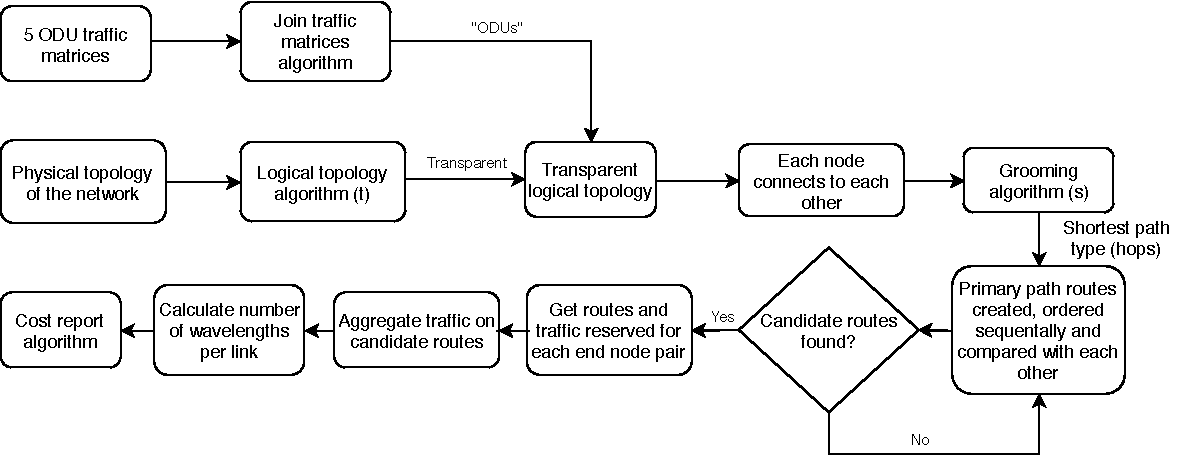
\includegraphics[width=16cm]{sdf/heuristic/transparent_survivability/figures/fluxogram_transparent_surv}
\caption{Fluxogram with the steps performed in the transparent without survivability transport mode approach.}
\label{fluxogram_transp_surv}
\end{figure}

\newpage
\subsubsection{Creation and join the traffic matrices}

\noindent
The first step is to create the traffic matrices based on the reference network \ref{Reference_Network_Topology}. In order to create the 5 traffic matrices in Net2Plan it is necessary the length of all the links and the total traffic used in this network, so later it is needed to define in Net2Plan the length in all end nodes and the total traffic depends on the value of traffic used (low traffic - 0.5 Tbit/s, medium traffic - 5 Tbit/s and high traffic - 10 Tbit/s). As you can see in the figure below, it is defined the path of the 5 ODUs and they will be aggregated in just one single ODU, making it possible to join all the demands in just one file and load it later into the network. This final resulting ODU joins the multiple traffic demands from all the traffic matrices previously created and, of course, the traffic demands will depend on the values used on the creation of the matrices (low, medium and high traffic).

\begin{figure}[H]
\centering
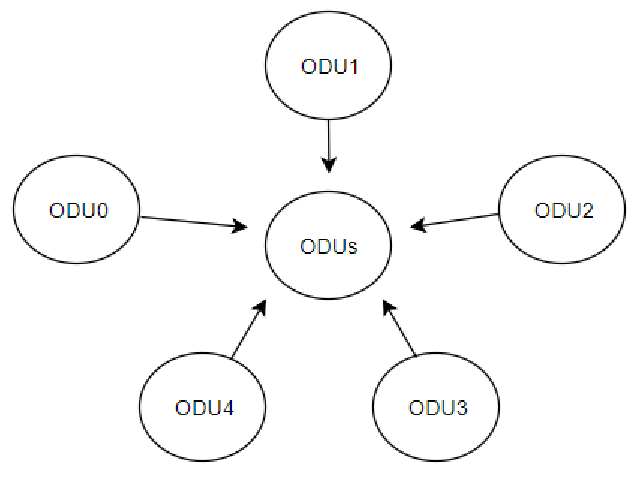
\includegraphics[width=9cm]{sdf/heuristic/transparent_survivability/figures/join_matrices_odus}
\caption{Join the 5 ODU traffic matrices into 1 single file "ODUs". The 5 traffic demands from the traffic matrices previously created are joined into 1 file to load it later on Net2Plan.}
\label{join_matrices_odus}
\end{figure}

\begin{figure}[H]
\centering
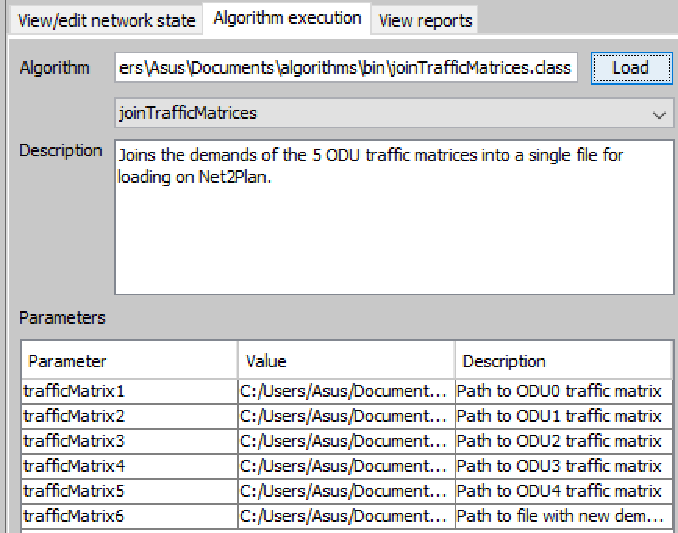
\includegraphics[width=11cm]{sdf/heuristic/transparent_survivability/figures/traffic_matrices}
\caption{Load of the join traffic matrices algorithm for the transparent transport mode on Net2Plan. It is defined the 5 paths to load the 5 ODU traffic matrices and the last path is the one where will be saved the file that joins all 5 the traffic demands.}
\label{traffic_matrices_transp_surv_ref}
\end{figure}

\newpage
\subsubsection{Creation of the physical topology}

\vspace{11pt}
The next step is to create the allowed physical topology of the network in Net2Plan. This network consists in 6 nodes and 8 bidirectional links. It is now also possible to define the length in all links. In the figure below it is shown the allowed physical topology in this transport mode.

\begin{figure}[H]
\centering
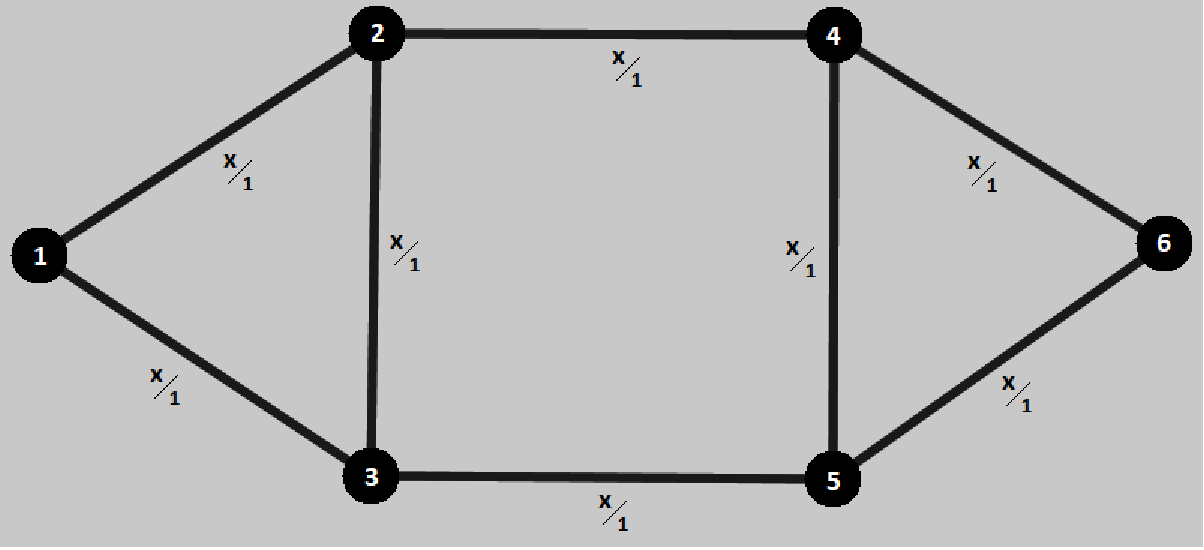
\includegraphics[width=13cm]{sdf/heuristic/transparent_survivability/figures/allowed_physical}
\caption{Allowed physical topology. The allowed physical topology is defined by the duct and sites in the field. It is assumed that each duct supports up to 1 bidirectional transmission system and each site supports up to 1 node.}
\label{allowed_physical_surv}
\end{figure}

\subsubsection{Creation of the logical topology}

\vspace{11pt}
It is now time to create the allowed logical topology. A network topology represents how the links and the nodes of the network interconnect with each other and the logical topology algorithm creates the logical topology on another layer. In the transparent transport mode each node connects to each other creating direct links between all nodes in the network. Going through all nodes, if a node has a different index from other one, then creates a shortest and direct link between them. These additions of links between end nodes are made in the new upper layer of the network. The respective demands are saved in the new upper layer and those demands from the lower layer are then removed. The lower layer is the physical layer of the network and it is now created a new upper layer which is the logical layer of the network and represents the logical topology of the transparent transport mode.

The allowed physical and optical topologies, the logical topologies for all ODUs and the resulting physical topology is shown in the next section below \ref{result_description_transparent_heuristic_surv} for the three traffic scenarios. It is shown below three figures with the code in Java of the creation of the network logical topology, the load of the logical topology algorithm in Net2Plan and the resulting allowed optical topology for the transparent transport mode without survivability.

\begin{figure}[H]
\centering
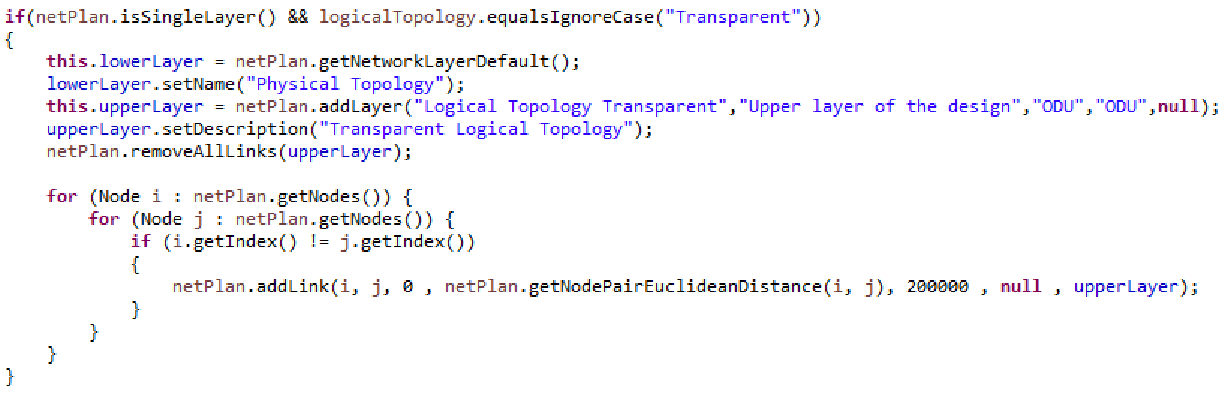
\includegraphics[width=15cm]{sdf/heuristic/transparent_survivability/figures/logical_topology_creation_transparent}
\caption{Java code of the logical topology approach for the transparent transport mode. The logical layer is created by adding direct links between all end nodes. The new layer is now the transparent logical topology of the network.}
\label{logical_topology_creation_transparent}
\end{figure}

\begin{figure}[H]
\centering
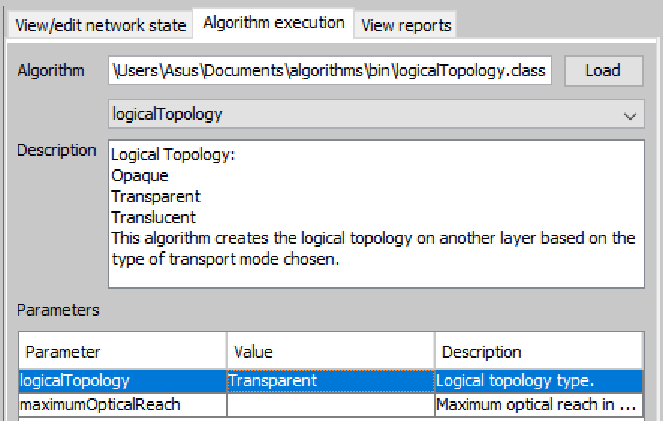
\includegraphics[width=11cm]{sdf/heuristic/transparent_survivability/figures/logical_topology_load_transparent}
\caption{Load of the logical topology algorithm for the transparent transport mode on Net2Plan.}
\label{logical_topology_load_transparent}
\end{figure}

\begin{figure}[H]
\centering
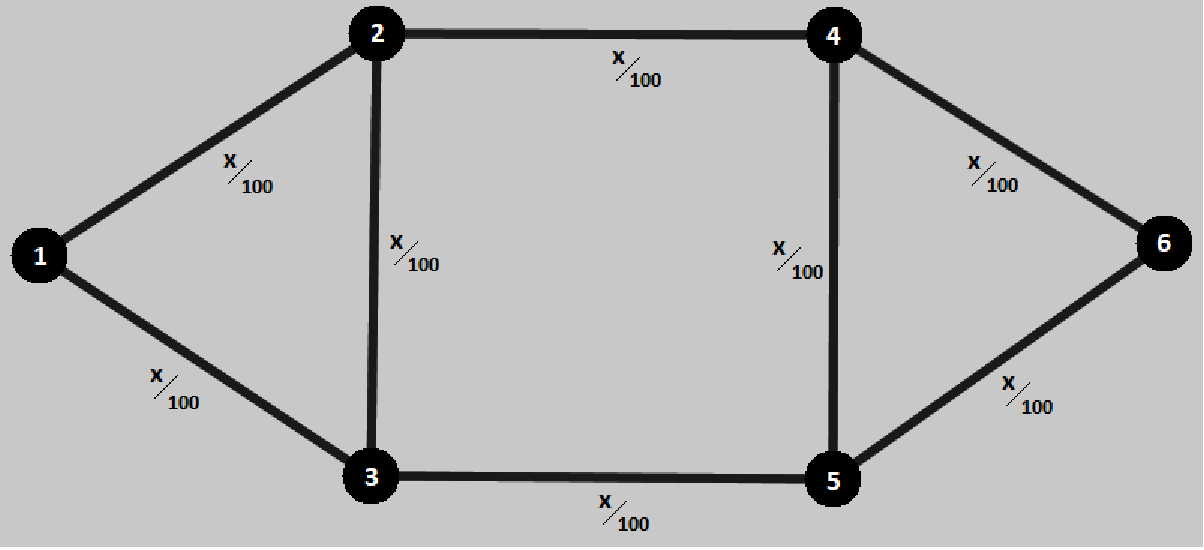
\includegraphics[width=13cm]{sdf/heuristic/transparent_survivability/figures/allowed_optical}
\caption{Allowed optical topology. It is assumed that each connections between demands supports up to 100 lightpaths.}
\label{allowed_optical_surv_transparent}
\end{figure}

\subsubsection{Creation of routes and aggregation of traffic}

\vspace{11pt}
After a network topology is created, it is now time to set the routing algorithm. In the transparent without survivability transport mode the routing algorithm is similar with the one used in opaque transport mode. It starts with going through all the demands and nodes which have different index between them (end nodes), create bidirectional routes (in this case the primary paths) based on the shortest path Dijkstra algorithm and then search the candidate routes for the respective demand. In this report it is used the shortest path type in hops. These routes are ordered sequentially and the shortest one per each demand is the primary path. The demands from the lower layer are removed and then saved in the upper layer. After this step, the routes are saved to a "Set" \ of routes and in each link of end nodes it is set the traffic demands into these routes that will integrate the whole network.

\begin{figure}[H]
\centering
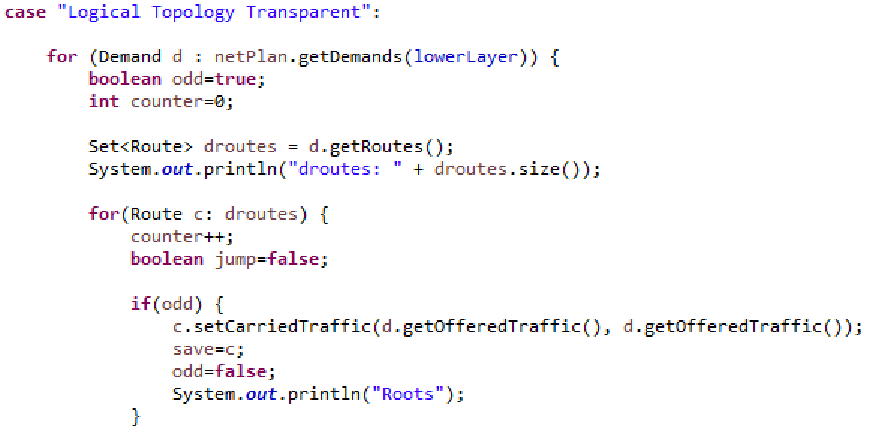
\includegraphics[width=14cm]{sdf/heuristic/transparent_survivability/figures/grooming_transparent_surv1}
\caption{Creation of routes and aggregation of traffic for the transparent without survivability transport mode. The candidate routes are searched by the shortest path type and the offered traffic demands are set into these routes.}
\label{grooming_transparent_surv1}
\end{figure}

\begin{figure}[H]
\centering
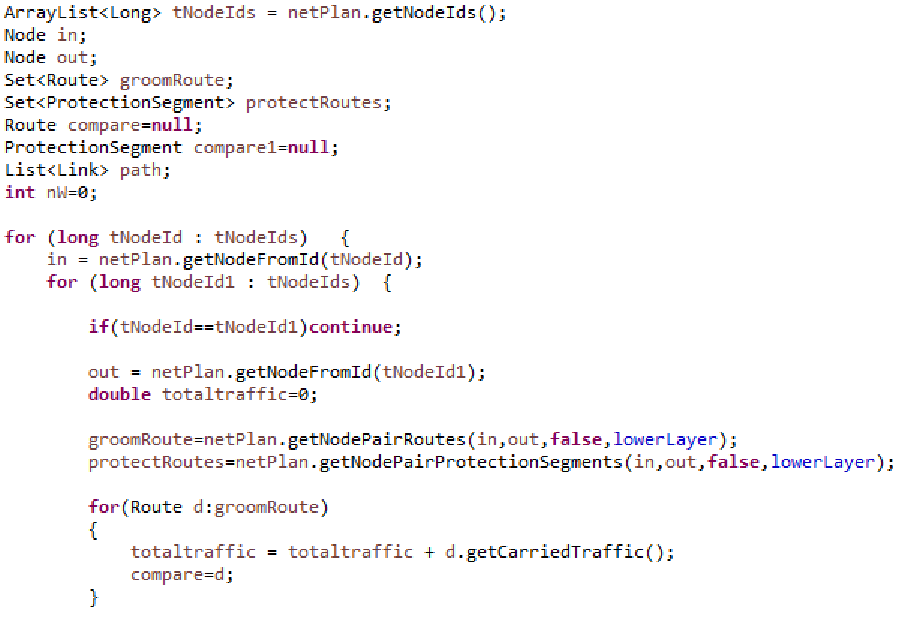
\includegraphics[width=14cm]{sdf/heuristic/transparent_survivability/figures/grooming_transparent_surv2}
\caption{Creation of routes and aggregation of traffic for the transparent without survivability transport mode. The traffic demands are set in the candidate primary path routes found earlier.}
\label{grooming_transparent_surv2}
\end{figure}

\begin{table}[H]
\centering
\begin{tabular}{|| c | c ||}
 \hline
 Function & Definition \\
 \hline\hline
 netPlan.getDemands(lowerLayer) & Returns the array of demands for the lower layer. \\
 \hline
 d.getRoutes() & Returns all the routes associated to the demand "d". \\
 \hline
 c.setCarriedTraffic() & \makecell{Sets the route carried traffic and the occupied capacity\\in the links, setting it up to be the same in all links.} \\
 \hline
 d.getOfferedTraffic() & Returns the offered traffic of the demand "d". \\
 \hline
 netPlan.getNodeIds() & Returns the array of the nodes' indexes. \\
 \hline
 netPlan.getNodeFromId(tNodeId) & Returns the node with the index "tNodeId". \\
 \hline
 \makecell{netPlan.getNodePairRoutes\\(in,out,false,lowerLayer)} & Returns the routes at "lowerLayer" \ from nodes "in" \ and "out". \\
 \hline
\end{tabular}
\caption{Table with the description of the main functions in the creation of routes and aggregation of traffic in the grooming algorithm.}
\label{grooming_table_variables_transparent}
\end{table}

\subsubsection{Calculation of the number of wavelengths per link}

\vspace{11pt}
The final step of the routing and grooming algorithms is to calculate the number of wavelengths per link for the whole network. This is the last and an important step because with the number of wavelengths per link in the network, it is possible to calculate other network components. In the transparent transport mode, as in the figure below shows, the algorithm starts with going through all the nodes which have different index between them (end nodes) and in all the links that crosses between these pairs of nodes is reserved a link capacity based on the previous traffic aggregation. The total carried traffic in the link including protection and non-protection segments will be divided by the wavelength capacity and it is now possible to obtain the number of wavelengths per link.

\begin{figure}[H]
\centering
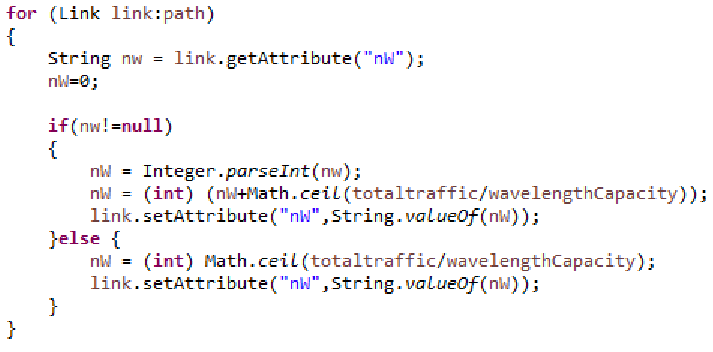
\includegraphics[width=15cm]{sdf/heuristic/transparent_survivability/figures/grooming_transparent_surv3}
\caption{Calculation of the number of wavelengths per link for the transparent transport mode. The link capacity is reserved based on the previous traffic aggregation.}
\label{grooming_transparent_surv3}
\end{figure}

\begin{figure}[H]
\centering
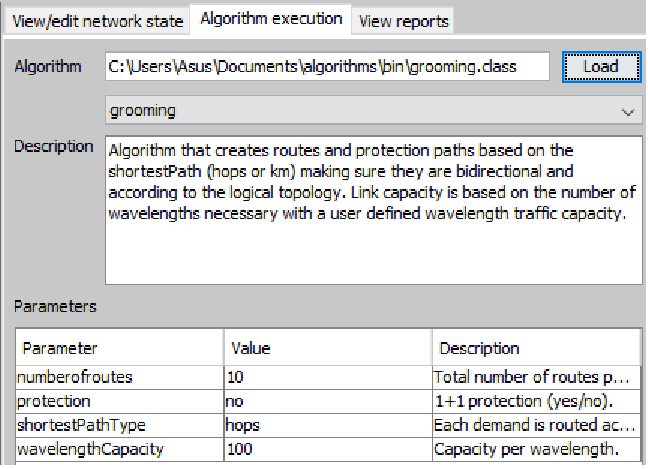
\includegraphics[width=11cm]{sdf/heuristic/transparent_survivability/figures/grooming_transparent_surv4}
\caption{Load of the grooming algorithm for the transparent without survivability transport mode. The total number of routes per demand is set to 100, the user can define if the model is with or without protection, the shortest path type is set to "hops" \ and the capacity per wavelength is used 100 optical channels.}
\label{grooming_transparent_surv4}
\end{figure}

\subsubsection{Network cost report}

\vspace{11pt}
In order to obtain the network CAPEX results, the formulas needed to calculate the network elements and that are demonstrated previously in the beginning of this section \ref{heuristic_Transp_Survivability} were "translated" \ into Java code in a cost report algorithm. This algorithm can be loaded in Net2Plan and calculates and shows in tables the network CAPEX and also the per-link and per-node information with more details.

\begin{figure}[H]
\centering
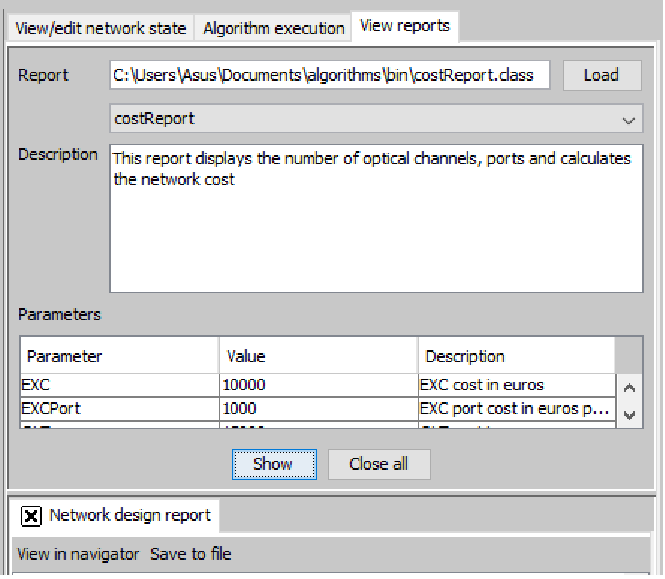
\includegraphics[width=11cm]{sdf/heuristic/transparent_survivability/figures/cost_report_transparent}
\caption{Load of the cost report algorithm on Net2Plan. The result view is an HTML page with the network optical and electrical components and their costs.}
\label{cost_report_transparent}
\end{figure}

\subsubsection{Result description}\label{result_description_transparent_heuristic_surv}

It is already known all the necessary formulas to obtain the CAPEX value for the reference network \ref{Reference_Network_Topology}. As described in the subsection of the network traffic \ref{Reference_Network_Traffic}, it is necessary to obtain three different values of CAPEX for the low (0.5 Tbit/s), medium (5 Tbit/s) and high (10 Tbit/s) traffic. It is used a network software program called Net2Plan which can design the traffic matrices, create all the network topologies, simulate the algorithms into the network implemented in the programming software called Eclipse and analyze the results obtained.\\
In this chapter will be demonstrated the results by Vasco's heuristics from 2016. In each of the three traffic scenarios, it will be shown the network topologies followed by the table with the CAPEX value of the network.\\

\noindent
\textbf{Low Traffic Scenario:}\\

In this scenario we have to take into account the traffic calculated in \ref{low_scenario}. In a first phase we will show the various existing topologies of the network. The first are the allowed topologies, physical and optical topologies, the second are the logical topology for all ODUs and finally the resulting physical topology.\\

\begin{figure}[H]
\centering
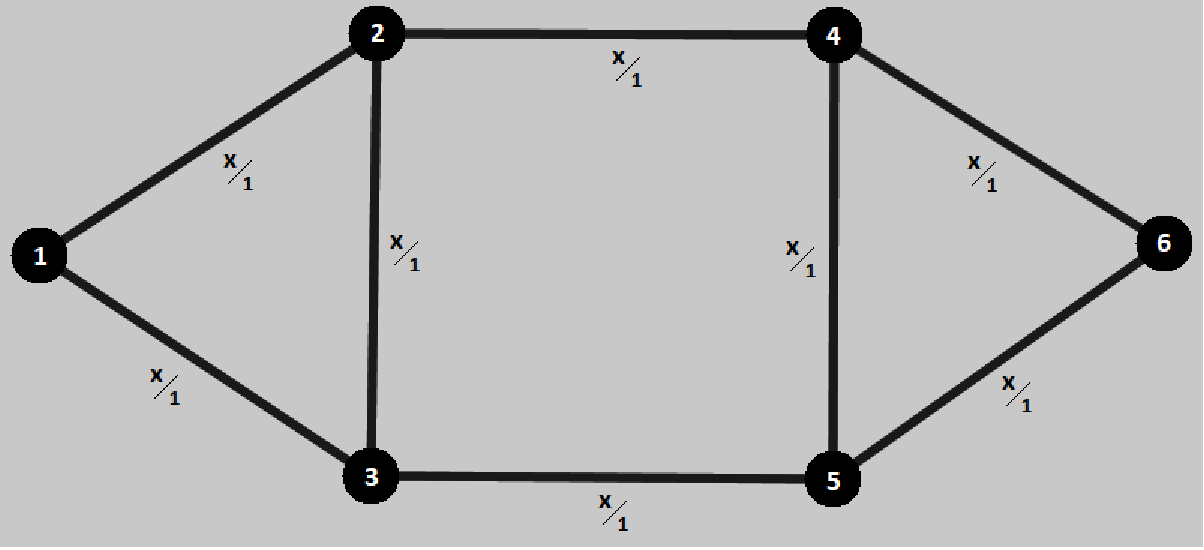
\includegraphics[width=13cm]{sdf/heuristic/transparent_survivability/figures/allowed_physical}
\caption{Allowed physical topology. The allowed physical topology is defined by the duct and sites in the field. It is assumed that each duct supports up to 1 bidirectional transmission system and each site supports up to 1 node.}
\label{allowed_physical_surv_ref_low_heuristic_transparent}
\end{figure}

\begin{figure}[H]
\centering
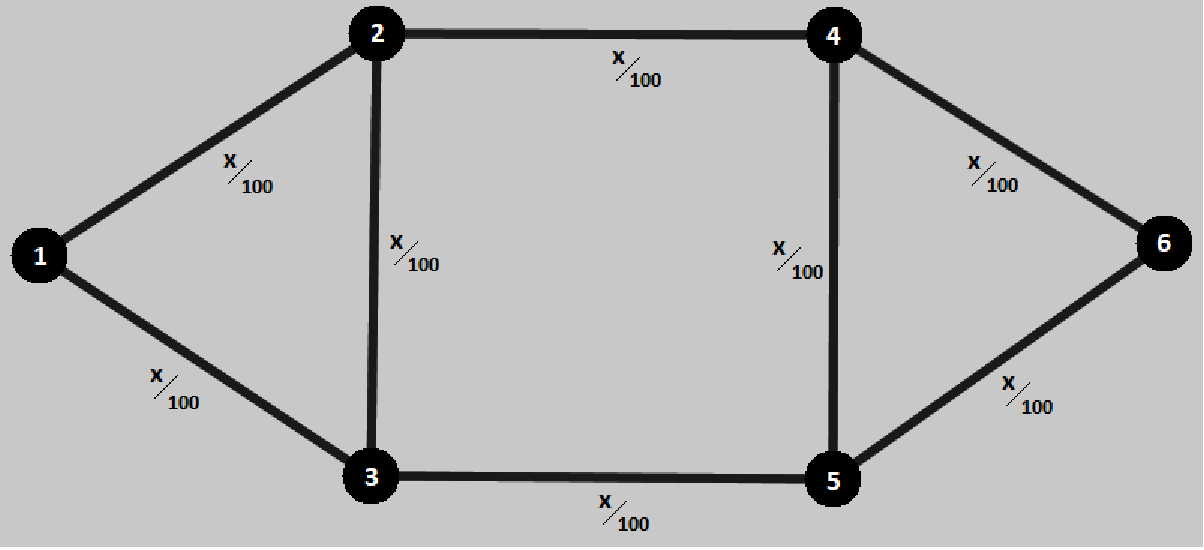
\includegraphics[width=13cm]{sdf/heuristic/transparent_survivability/figures/allowed_optical}
\caption{Allowed optical topology. The allowed optical topology is defined by the transport mode (transparent transport mode in this case). It is assumed that each connections between demands supports up to 100 lightpaths.}
\label{allowed_optical_surv_ref_low_heuristic_transparent}
\end{figure}

\begin{figure}[H]
\centering
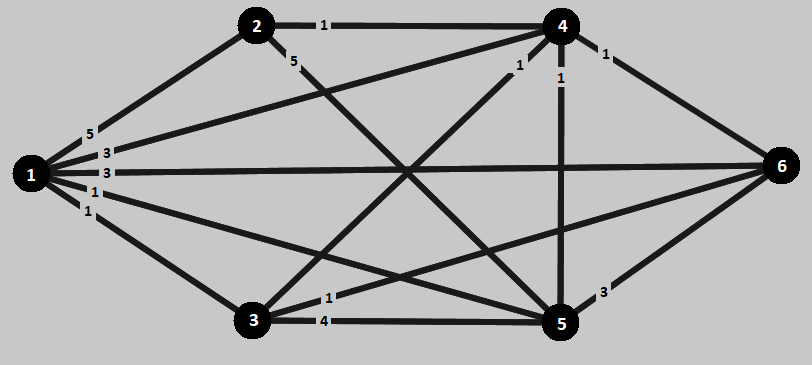
\includegraphics[width=13cm]{sdf/heuristic/transparent_survivability/figures/logical_topology_odu0_low}
\caption{ODU0 logical topology defined by the ODU0 traffic matrix.}
\label{logical_ODU0_surv_ref_low_heuristic_transparent}
\end{figure}

\begin{figure}[H]
\centering
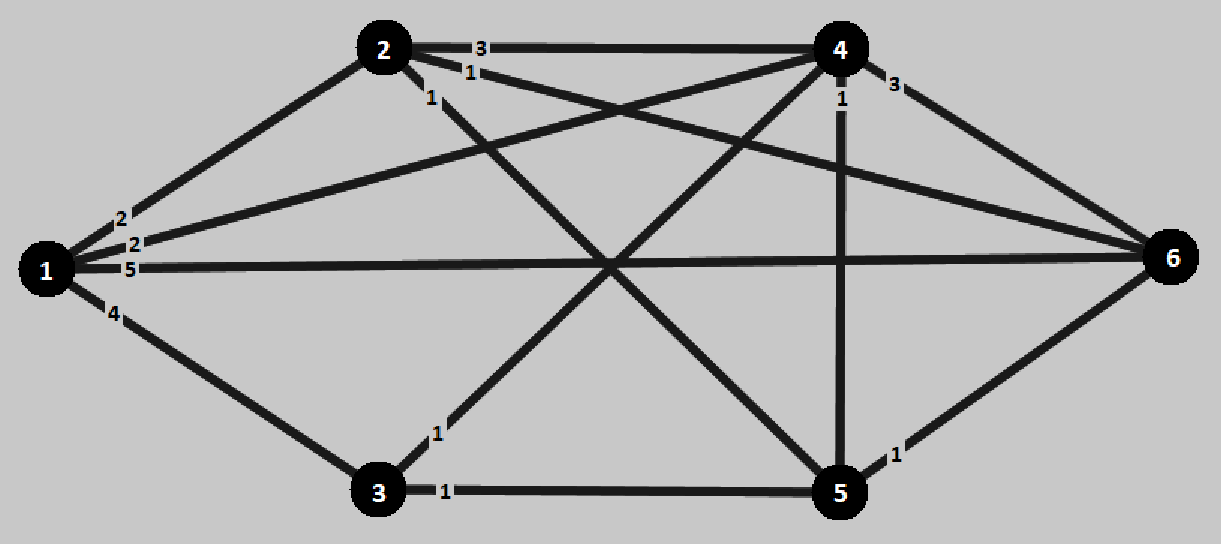
\includegraphics[width=13cm]{sdf/heuristic/transparent_survivability/figures/logical_topology_odu1_low}
\caption{ODU1 logical topology defined by the ODU1 traffic matrix.}
\label{logical_ODU1_surv_ref_low_heuristic_transparent}
\end{figure}

\begin{figure}[H]
\centering
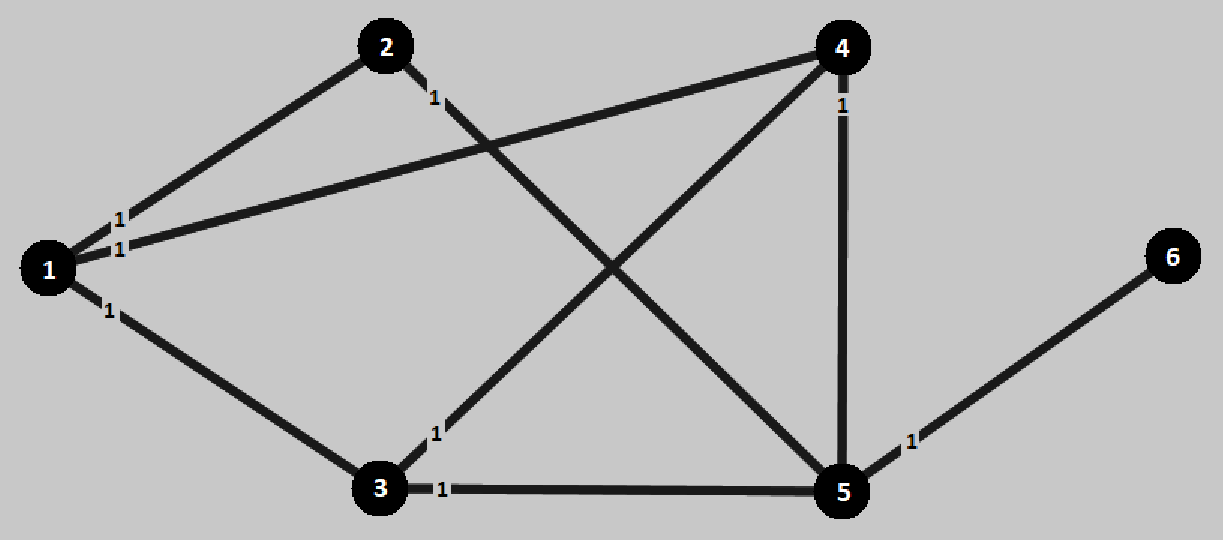
\includegraphics[width=13cm]{sdf/heuristic/transparent_survivability/figures/logical_topology_odu2_low}
\caption{ODU2 logical topology defined by the ODU2 traffic matrix.}
\label{logical_ODU2_surv_ref_low_heuristic_transparent}
\end{figure}

\begin{figure}[H]
\centering
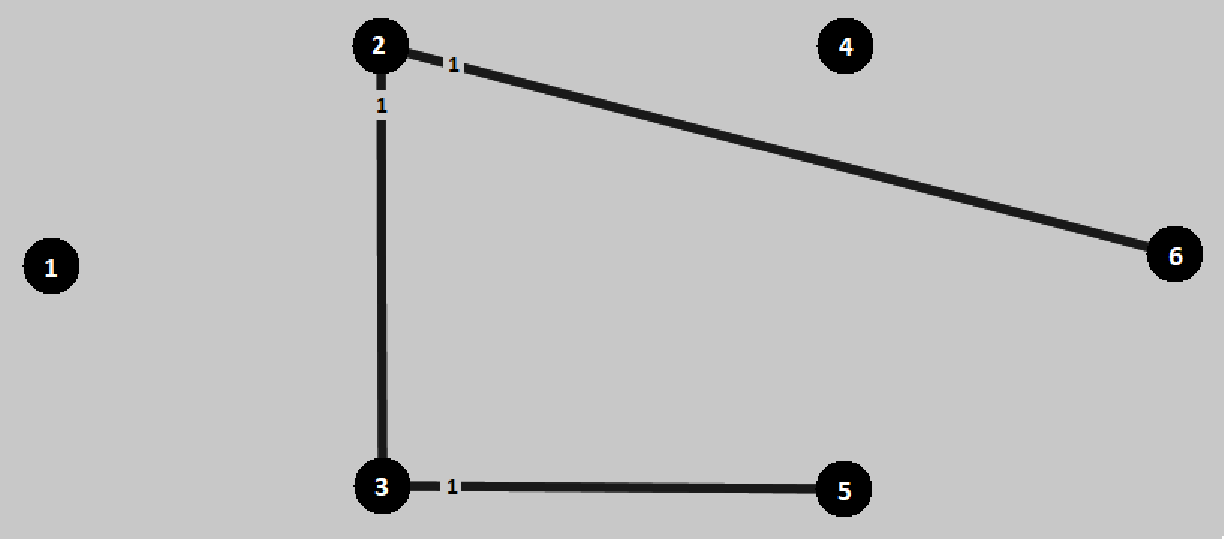
\includegraphics[width=13cm]{sdf/heuristic/transparent_survivability/figures/logical_topology_odu3_low}
\caption{ODU3 logical topology defined by the ODU3 traffic matrix.}
\label{logical_ODU3_surv_ref_low_heuristic_transparent}
\end{figure}

\begin{figure}[H]
\centering
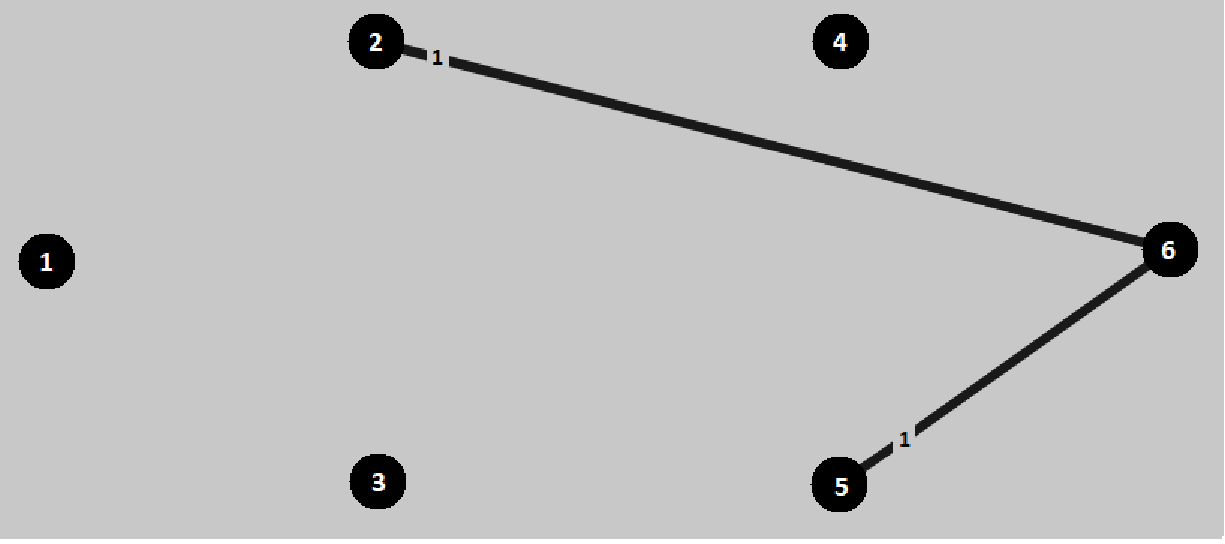
\includegraphics[width=13cm]{sdf/heuristic/transparent_survivability/figures/logical_topology_odu4_low}
\caption{ODU4 logical topology defined by the ODU4 traffic matrix.}
\label{logical_ODU4_surv_ref_low_heuristic_transparent}
\end{figure}

\begin{figure}[H]
\centering
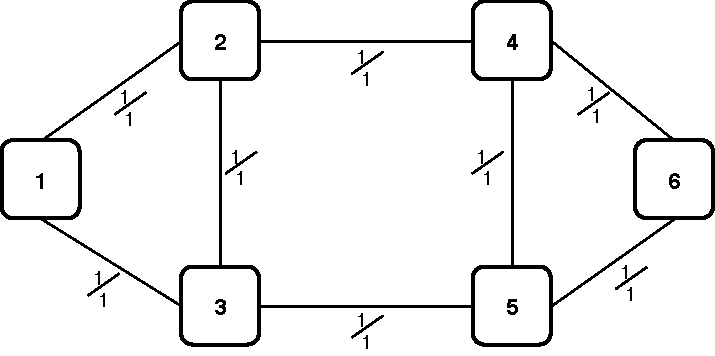
\includegraphics[width=13cm]{sdf/heuristic/transparent_survivability/figures/physical_topology}
\caption{Physical topology after dimensioning.}
\label{physical_topology_surv_ref_low_heuristic_transparent}
\end{figure}

Following all the steps mentioned in the \ref{net2plan_guide}, applying the routing and grooming heuristic algorithms in the Net2Plan software and using all the data referring to this scenario, the obtained result for the Vasco's heuristics can be consulted in the following table \ref{scripttransp_surv_ref_low_heuristic}.\\

\begin{table}[H]
\centering
\begin{tabular}{|| c | c | c | c | c | c | c ||}
 \hline
 \multicolumn{7}{|| c ||}{CAPEX of the Network} \\
 \hline
 \hline
 \multicolumn{3}{|| c |}{ } & Quantity & Unit Price & Cost & Total \\
 \hline
 \multirow{3}{*}{\makecell{Link \\ Cost}} & \multicolumn{2}{ c |}{OLTs} & 16 & 15 000 \euro & 240 000 \euro & \multirow{3}{*}{26 520 000 \euro} \\ \cline{2-6}
 & \multicolumn{2}{ c |}{100 Gbits/s Transceivers} & 52 & 5 000 \euro/Gbit/s & 26 000 000 \euro & \\ \cline{2-6}
 & \multicolumn{2}{ c |}{Amplifiers} & 70 & 4 000 \euro & 280 000 \euro & \\
 \hline
 \multirow{10}{*}{\makecell{Node \\ Cost}} & \multirow{7}{*}{Electrical} & EXCs & 6 & 10 000 \euro & 60 000 \euro & \multirow{10}{*}{3 797 590 \euro} \\ \cline{3-6}
  & & ODU0 Ports & 60 & 10 \euro/port & 600 \euro & \\ \cline{3-6}
 & & ODU1 Ports & 50 & 15 \euro/port & 750 \euro & \\ \cline{3-6}
 & & ODU2 Ports & 16 & 30 \euro/port & 480 \euro & \\ \cline{3-6}
 & & ODU3 Ports & 6 & 60 \euro/port & 360 \euro & \\ \cline{3-6}
 & & ODU4 Ports & 4 & 100 \euro/port & 400 \euro & \\ \cline{3-6}
 & & Transponders & 34 & 100 000 \euro/port & 3 400 000 \euro & \\ \cline{2-6}
 & \multirow{3}{*}{Optical} & OXCs & 6 & 20 000 \euro & 120 000 \euro & \\ \cline{3-6}
 & & Line Ports & 52 & 2 500 \euro/port & 130 000 \euro & \\ \cline{3-6}
 & & Add Ports & 34 & 2 500 \euro/port & 85 000 \euro & \\
 \hline
 \multicolumn{6}{|| c |}{Total Network Cost} & 30 317 590 \euro \\
\hline
\end{tabular}
\caption{Table with detailed description of CAPEX of Vasco's 2016 results.}
\label{scripttransp_surv_ref_low_heuristic}
\end{table}

\vspace{17pt}
All the values calculated in the previous table were obtained through the equations \ref{Capex_Link_heuristic} and \ref{Capex_Node_heuristic} referred to in section \ref{Heuristic_CAPEX}, but for a more detailed analysis we created table \ref{formulas_transp_heuristic} where we can see how all the parameters are calculated individually. \\

\begin{table}[h!]
\centering
\begin{tabular}{|| c | c ||}
 \hline
  & Equation used to calculate the cost \\ \hline
 OLTs & \(\displaystyle 2 \sum_{i=1}^{N}\sum_{j=i+1}^{N} L_{ij} \gamma_0^{OLT} \) \\ \hline
 Transceivers & \(\displaystyle 2 \sum_{i=1}^{N}\sum_{j=i+1}^{N} L_{ij} f_{ij}^{od} \gamma_1^{OLT} \tau \) \\ \hline
 Amplifiers & \(\displaystyle 2 \sum_{i=1}^{N}\sum_{j=i+1}^{N} L_{ij} N^R_{ij} c^R \) \\ \hline
 EXCs & \(\displaystyle \sum_{n=1}^N N_{exc,n} \gamma_{e0} \) \\ \hline
 ODU0 Port & \(\displaystyle \sum_{n=1}^{N} \sum_{d=1}^{N} N_{exc,n} D_{nd,0} \gamma_{e1,0} \) \\ \hline
 ODU1 Port & \(\displaystyle \sum_{n=1}^{N} \sum_{d=1}^{N} N_{exc,n} D_{nd,1} \gamma_{e1,1} \) \\ \hline
 ODU2 Port & \(\displaystyle \sum_{n=1}^{N} \sum_{d=1}^{N} N_{exc,n} D_{nd,2} \gamma_{e1,2} \)\\ \hline
 ODU3 Port & \(\displaystyle \sum_{n=1}^{N} \sum_{d=1}^{N} N_{exc,n} D_{nd,3} \gamma_{e1,3} \) \\ \hline
 ODU4 Port & \(\displaystyle \sum_{n=1}^{N} \sum_{d=1}^{N} N_{exc,n} D_{nd,4} \gamma_{e1,4} \) \\ \hline
 LR Transponders & \(\displaystyle \sum_{n=1}^{N} \sum_{j=1}^{N} N_{exc,n} \lambda_{od} \gamma_{e1,-1} \) \\ \hline
 OXCs & \(\displaystyle \sum_{n=1}^N N_{oxc,n} \gamma_{o0} \) \\ \hline
 Add Port & \(\displaystyle \sum_{n=1}^{N} \sum_{j=1}^{N} N_{oxc,n} \lambda_{od} \gamma_{o1} \) \\ \hline
 Line Port & \(\displaystyle \sum_{n=1}^{N} \sum_{j=1}^{N} N_{oxc,n} f_{ij}^{od} \gamma_{o1} \) \\ \hline
 CAPEX & The final cost is calculated by summing all previous results. \\
 \hline
 \end{tabular}
\caption{Table with description of calculation}
\label{formulas_transp_heuristic}
\end{table}

\noindent
\textbf{Medium Traffic Scenario:}\\

In this scenario we have to take into account the traffic calculated in \ref{medium_traffic_scenario}. In a first phase we will show the various existing topologies of the network. The first are the allowed topologies, physical and optical topologies, the second are the logical topology for all ODUs and finally the resulting physical topology.\\

\begin{figure}[H]
\centering
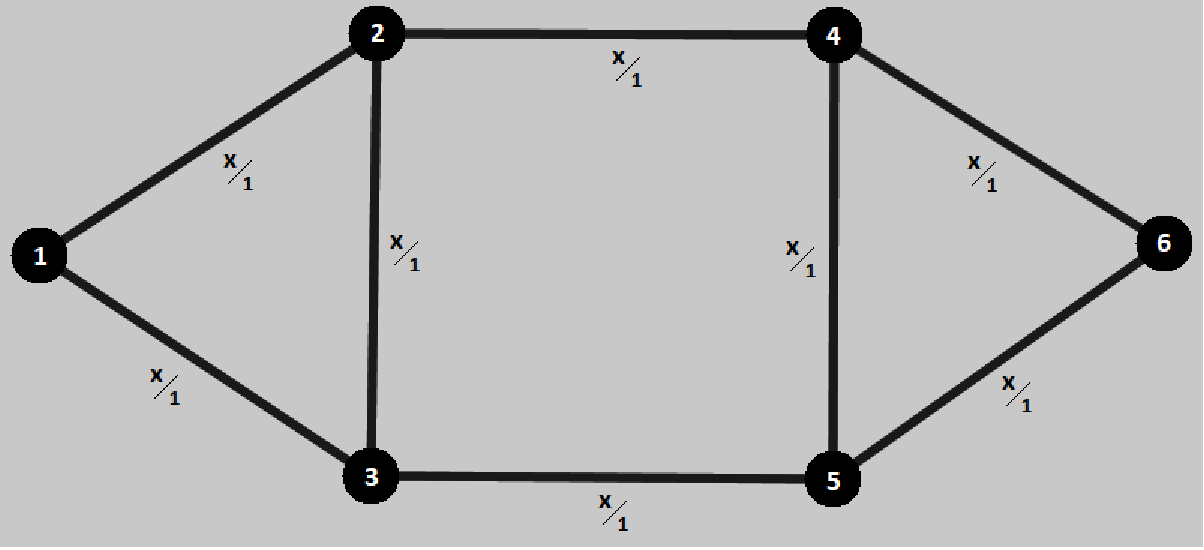
\includegraphics[width=13cm]{sdf/heuristic/transparent_survivability/figures/allowed_physical}
\caption{Allowed physical topology. The allowed physical topology is defined by the duct and sites in the field. It is assumed that each duct supports up to 1 bidirectional transmission system and each site supports up to 1 node.}
\label{allowed_physical_surv_ref_medium_heuristic_transparent}
\end{figure}

\begin{figure}[H]
\centering
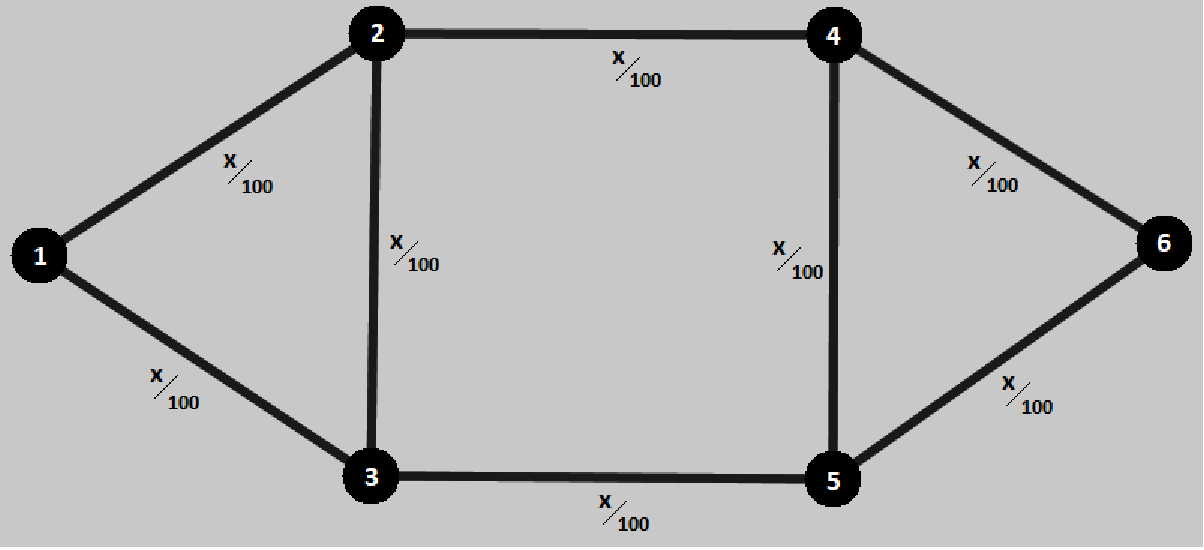
\includegraphics[width=13cm]{sdf/heuristic/transparent_survivability/figures/allowed_optical}
\caption{Allowed optical topology. The allowed optical topology is defined by the transport mode (transparent transport mode in this case). It is assumed that each connections between demands supports up to 100 lightpaths.}
\label{allowed_optical_surv_ref_medium_heuristic_transparent}
\end{figure}

\begin{figure}[H]
\centering
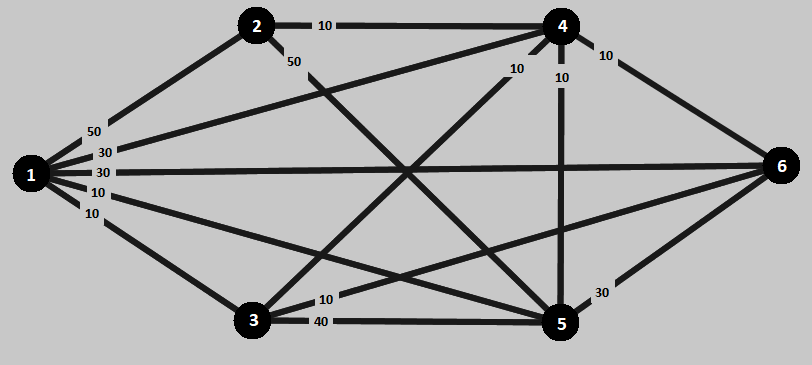
\includegraphics[width=13cm]{sdf/heuristic/transparent_survivability/figures/logical_topology_odu0_medium}
\caption{ODU0 logical topology defined by the ODU0 traffic matrix.}
\label{logical_ODU0_surv_ref_medium_heuristic_transparent}
\end{figure}

\begin{figure}[H]
\centering
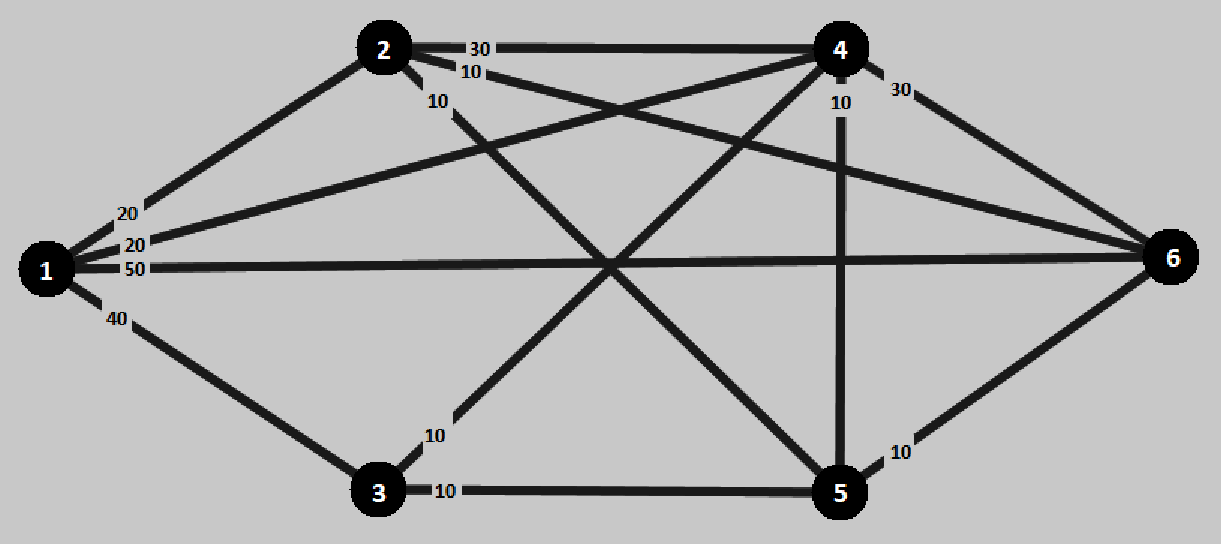
\includegraphics[width=13cm]{sdf/heuristic/transparent_survivability/figures/logical_topology_odu1_medium}
\caption{ODU1 logical topology defined by the ODU1 traffic matrix.}
\label{logical_ODU1_surv_ref_medium_heuristic_transparent}
\end{figure}

\begin{figure}[H]
\centering
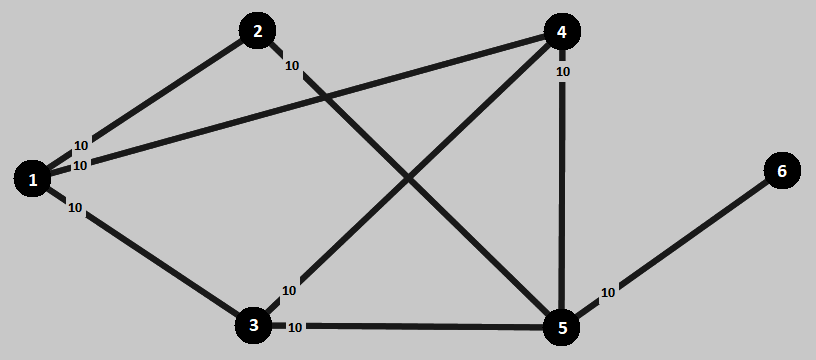
\includegraphics[width=13cm]{sdf/heuristic/transparent_survivability/figures/logical_topology_odu2_medium}
\caption{ODU2 logical topology defined by the ODU2 traffic matrix.}
\label{logical_ODU2_surv_ref_medium_heuristic_transparent}
\end{figure}

\begin{figure}[H]
\centering
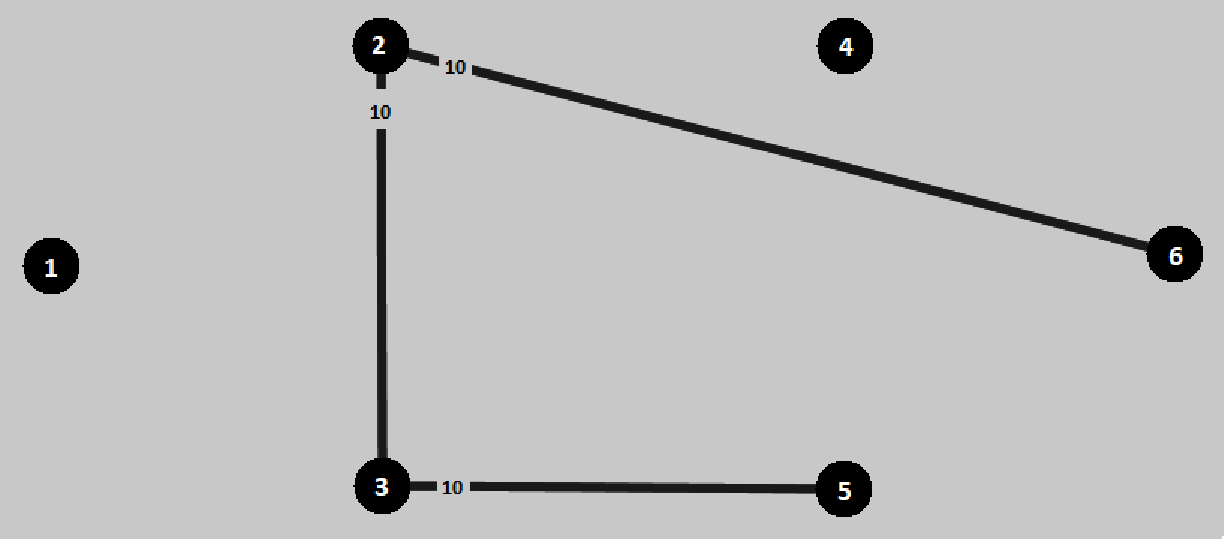
\includegraphics[width=13cm]{sdf/heuristic/transparent_survivability/figures/logical_topology_odu3_medium}
\caption{ODU3 logical topology defined by the ODU3 traffic matrix.}
\label{logical_ODU3_surv_ref_medium_heuristic_transparent}
\end{figure}

\begin{figure}[H]
\centering
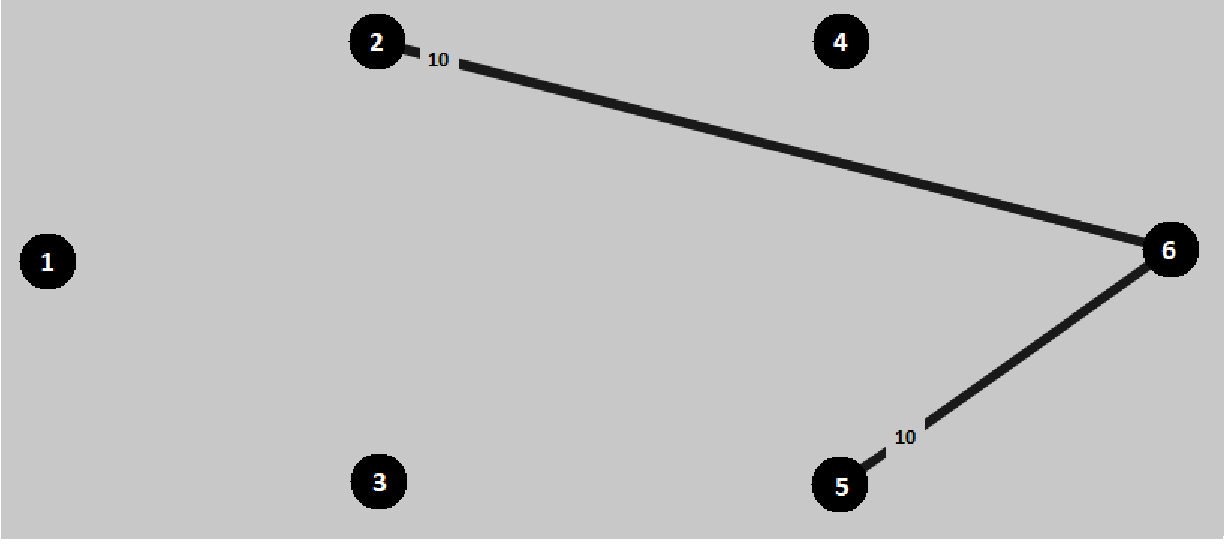
\includegraphics[width=13cm]{sdf/heuristic/transparent_survivability/figures/logical_topology_odu4_medium}
\caption{ODU4 logical topology defined by the ODU4 traffic matrix.}
\label{logical_ODU4_surv_ref_medium_heuristic_transparent}
\end{figure}

\begin{figure}[H]
\centering
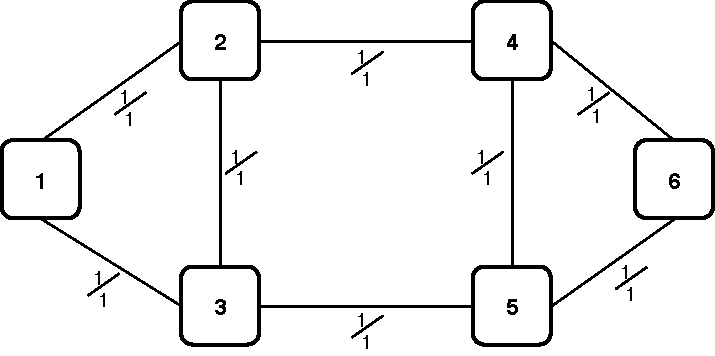
\includegraphics[width=13cm]{sdf/heuristic/transparent_survivability/figures/physical_topology}
\caption{Physical topology after dimensioning.}
\label{physical_topology_surv_ref_medium_heuristic_transparent}
\end{figure}

Following all the steps mentioned in the \ref{net2plan_guide}, applying the routing and grooming heuristic algorithms in the Net2Plan software and using all the data referring to this scenario, the obtained result for the Vasco's heuristics can be consulted in the following table \ref{scripttransp_surv_ref_medium_heuristic}. In table \ref{formulas_transp_heuristic} mentioned in previous scenario we can see how all the values were calculated. \\

\begin{table}[H]
\centering
\begin{tabular}{|| c | c | c | c | c | c | c ||}
 \hline
 \multicolumn{7}{|| c ||}{CAPEX of the Network} \\
 \hline
 \hline
 \multicolumn{3}{|| c |}{ } & Quantity & Unit Price & Cost & Total \\
 \hline
 \multirow{3}{*}{\makecell{Link \\ Cost}} & \multicolumn{2}{ c |}{OLTs} & 16 & 15 000 \euro & 240 000 \euro & \multirow{3}{*}{84 520 000 \euro} \\ \cline{2-6}
 & \multicolumn{2}{ c |}{100 Gbits/s Transceivers} & 168 & 5 000 \euro/Gbit/s & 84 000 000 \euro & \\ \cline{2-6}
 & \multicolumn{2}{ c |}{Amplifiers} & 70 & 4 000 \euro & 280 000 \euro & \\
 \hline
 \multirow{10}{*}{\makecell{Node \\ Cost}} & \multirow{7}{*}{Electrical} & EXCs & 6 & 10 000 \euro & 60 000 \euro & \multirow{10}{*}{15 180 900 \euro} \\ \cline{3-6}
 & & ODU0 Ports & 600 & 10 \euro/port & 6 000 \euro & \\ \cline{3-6}
 & & ODU1 Ports & 500 & 15 \euro/port & 7 500 \euro & \\ \cline{3-6}
 & & ODU2 Ports & 160 & 30 \euro/port & 4 800 \euro & \\ \cline{3-6}
 & & ODU3 Ports & 60 & 60 \euro/port & 3 600 \euro & \\ \cline{3-6}
 & & ODU4 Ports & 40 & 100 \euro/port & 4 000 \euro & \\ \cline{3-6}
 & & Transponders & 142 & 100 000 \euro/port & 14 200 000 \euro & \\ \cline{2-6}
 & \multirow{3}{*}{Optical} & OXCs & 6 & 20 000 \euro & 120 000 \euro & \\ \cline{3-6}
 & & Line Ports & 168 & 2 500 \euro/port & 420 000 \euro & \\ \cline{3-6}
 & & Add Ports & 142 & 2 500 \euro/port & 355 000 \euro & \\
 \hline
 \multicolumn{6}{|| c |}{Total Network Cost} & 99 700 900 \euro \\
\hline
\end{tabular}
\caption{Table with detailed description of CAPEX of Vasco's 2016 results.}
\label{scripttransp_surv_ref_medium_heuristic}
\end{table}

\noindent
\textbf{High Traffic Scenario:}\\

In this scenario we have to take into account the traffic calculated in \ref{high_traffic_scenario}. In a first phase we will show the various existing topologies of the network. The first are the allowed topologies, physical and optical topologies, the second are the logical topology for all ODUs and finally the resulting physical topology.\\

\begin{figure}[H]
\centering
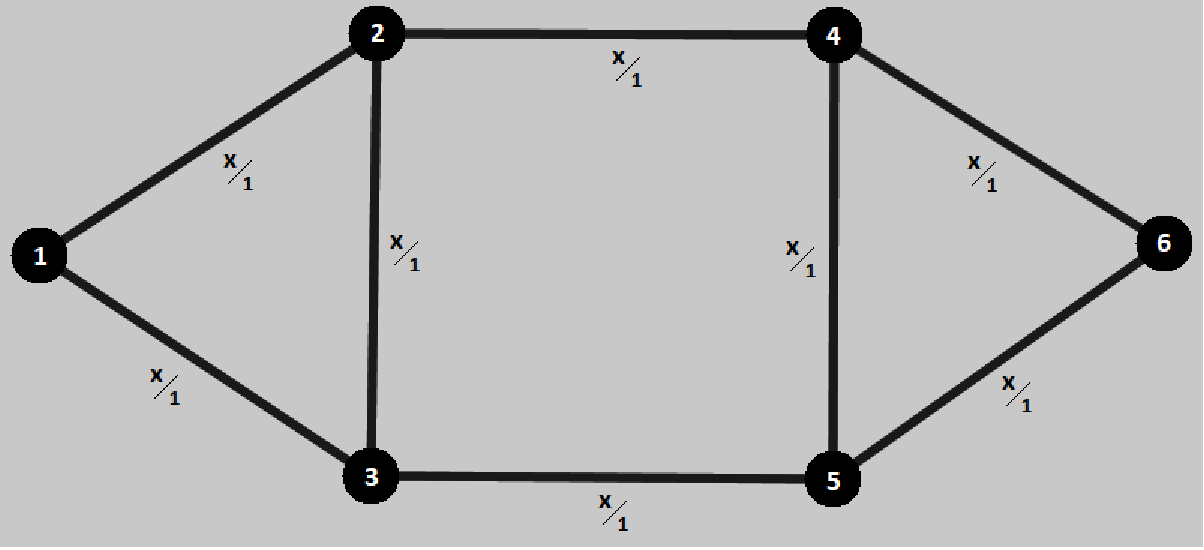
\includegraphics[width=13cm]{sdf/heuristic/transparent_survivability/figures/allowed_physical}
\caption{Allowed physical topology. The allowed physical topology is defined by the duct and sites in the field. It is assumed that each duct supports up to 1 bidirectional transmission system and each site supports up to 1 node.}
\label{allowed_physical_surv_ref_high_heuristic_transparent}
\end{figure}

\begin{figure}[H]
\centering
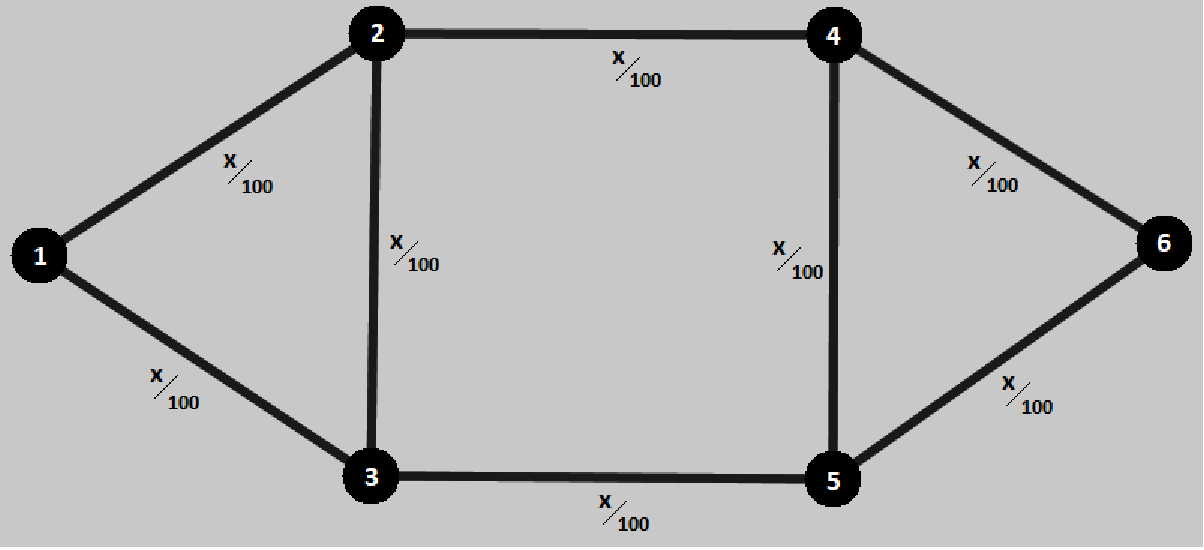
\includegraphics[width=13cm]{sdf/heuristic/transparent_survivability/figures/allowed_optical}
\caption{Allowed optical topology. The allowed optical topology is defined by the transport mode (transparent transport mode in this case). It is assumed that each connections between demands supports up to 100 lightpaths.}
\label{allowed_optical_surv_ref_high_heuristic_transparent}
\end{figure}

\begin{figure}[H]
\centering
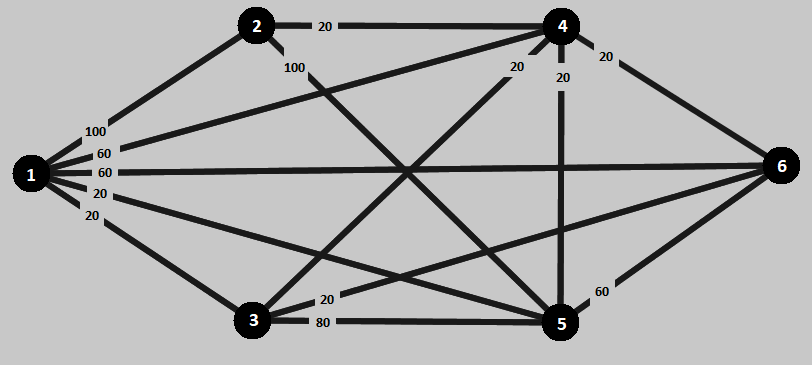
\includegraphics[width=13cm]{sdf/heuristic/transparent_survivability/figures/logical_topology_odu0_high}
\caption{ODU0 logical topology defined by the ODU0 traffic matrix.}
\label{logical_ODU0_surv_ref_high_heuristic_transparent}
\end{figure}

\begin{figure}[H]
\centering
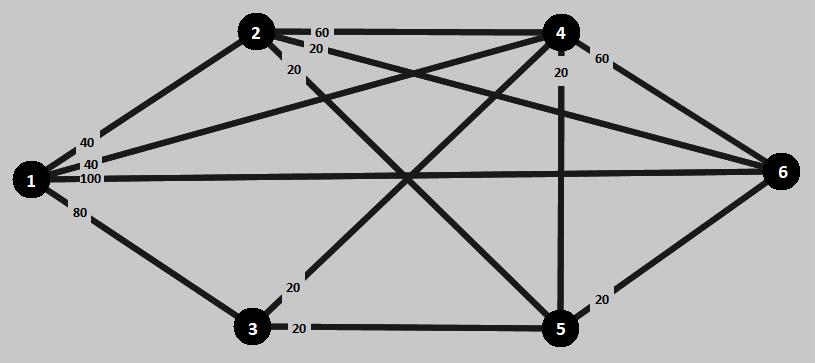
\includegraphics[width=13cm]{sdf/heuristic/transparent_survivability/figures/logical_topology_odu1_high}
\caption{ODU1 logical topology defined by the ODU1 traffic matrix.}
\label{logical_ODU1_surv_ref_high_heuristic_transparent}
\end{figure}

\begin{figure}[H]
\centering
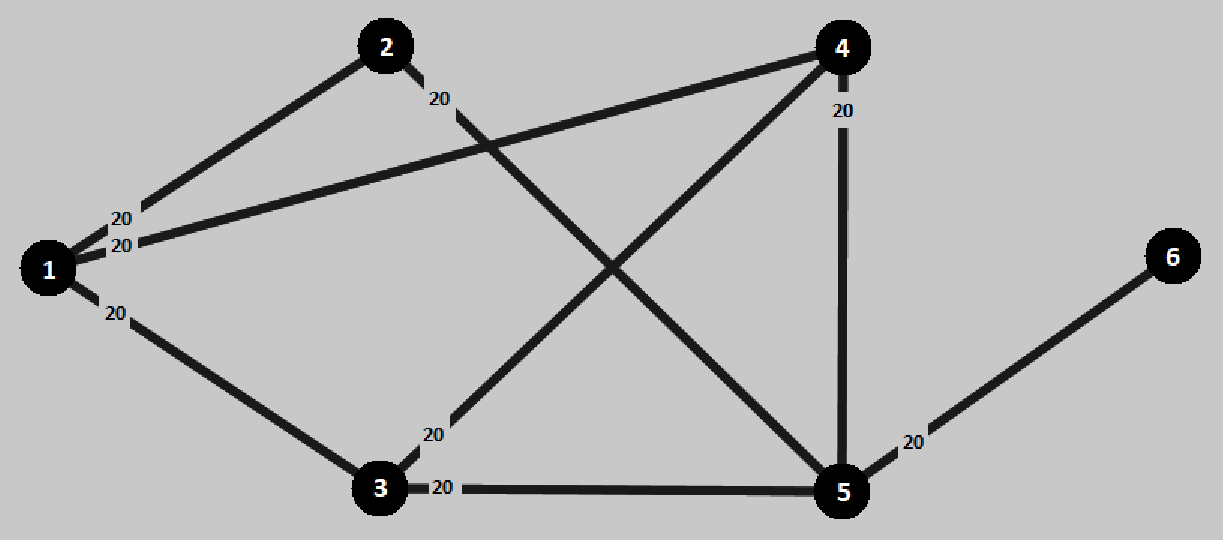
\includegraphics[width=13cm]{sdf/heuristic/transparent_survivability/figures/logical_topology_odu2_high}
\caption{ODU2 logical topology defined by the ODU2 traffic matrix.}
\label{logical_ODU2_surv_ref_high_heuristic_transparent}
\end{figure}

\begin{figure}[H]
\centering
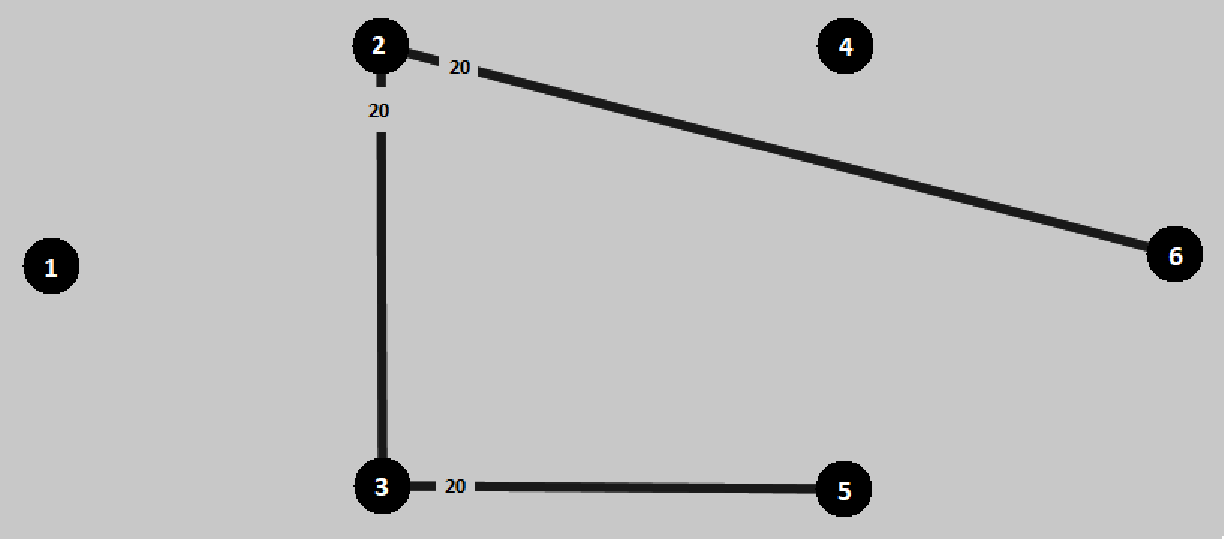
\includegraphics[width=13cm]{sdf/heuristic/transparent_survivability/figures/logical_topology_odu3_high}
\caption{ODU3 logical topology defined by the ODU3 traffic matrix.}
\label{logical_ODU3_surv_ref_high_heuristic_transparent}
\end{figure}

\begin{figure}[H]
\centering
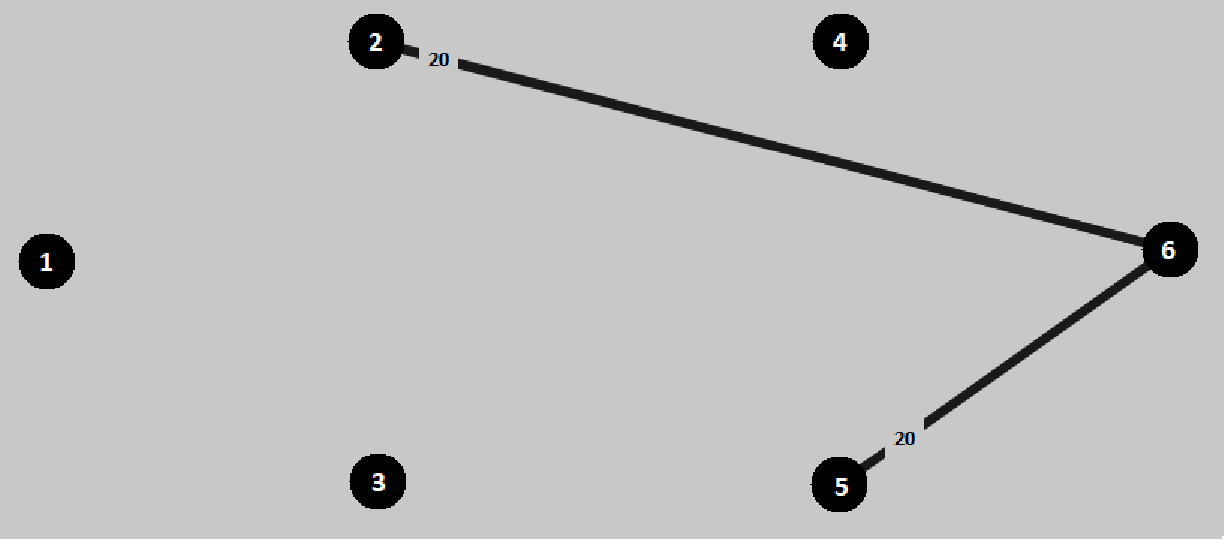
\includegraphics[width=13cm]{sdf/heuristic/transparent_survivability/figures/logical_topology_odu4_high}
\caption{ODU4 logical topology defined by the ODU4 traffic matrix.}
\label{logical_ODU4_surv_ref_high_heuristic_transparent}
\end{figure}

\begin{figure}[H]
\centering
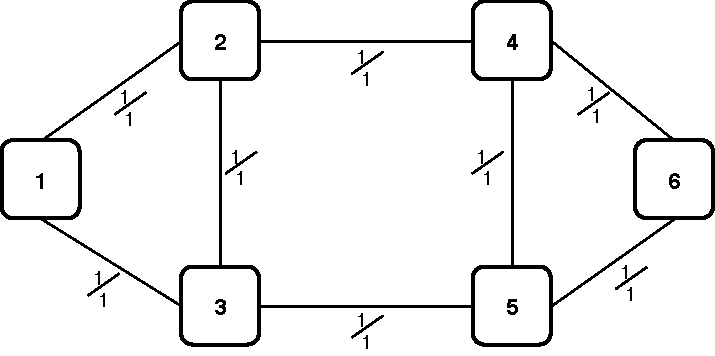
\includegraphics[width=13cm]{sdf/heuristic/transparent_survivability/figures/physical_topology}
\caption{Physical topology after dimensioning.}
\label{physical_topology_surv_ref_high_heuristic_transparent}
\end{figure}

Following all the steps mentioned in the \ref{net2plan_guide}, applying the routing and grooming heuristic algorithms in the Net2Plan software and using all the data referring to this scenario, the obtained result for the Vasco's heuristics can be consulted in the following table \ref{scripttransp_surv_ref_high_heuristic}. In table \ref{formulas_transp_heuristic} mentioned in previous scenario we can see how all the values were calculated. \\

\begin{table}[H]
\centering
\begin{tabular}{|| c | c | c | c | c | c | c ||}
 \hline
 \multicolumn{7}{|| c ||}{CAPEX of the Network} \\
 \hline
 \hline
 \multicolumn{3}{|| c |}{ } & Quantity & Unit Price & Cost & Total \\
 \hline
 \multirow{3}{*}{\makecell{Link \\ Cost}} & \multicolumn{2}{ c |}{OLTs} & 16 & 15 000 \euro & 240 000 \euro & \multirow{3}{*}{157 520 000 \euro} \\ \cline{2-6}
 & \multicolumn{2}{ c |}{100 Gbits/s Transceivers} & 314 & 5 000 \euro/Gbit/s & 157 000 000 \euro & \\ \cline{2-6}
 & \multicolumn{2}{ c |}{Amplifiers} & 70 & 4 000 \euro & 280 000 \euro & \\
 \hline
 \multirow{10}{*}{\makecell{Node \\ Cost}} & \multirow{7}{*}{Electrical} & EXCs & 6 & 10 000 \euro & 60 000 \euro & \multirow{10}{*}{28 486 800 \euro} \\ \cline{3-6}
  & & ODU0 Ports & 1 200 & 10 \euro/port & 12 000 \euro & \\ \cline{3-6}
 & & ODU1 Ports & 1 000 & 15 \euro/port & 15 000 \euro & \\ \cline{3-6}
 & & ODU2 Ports & 320 & 30 \euro/port & 9 600 \euro & \\ \cline{3-6}
 & & ODU3 Ports & 120 & 60 \euro/port & 7 200 \euro & \\ \cline{3-6}
 & & ODU4 Ports & 80 & 100 \euro/port & 8 000 \euro & \\ \cline{3-6}
 & & Transponders & 268 & 100 000 \euro/port & 26 800 000 \euro & \\ \cline{2-6}
 & \multirow{3}{*}{Optical} & OXCs & 6 & 20 000 \euro & 120 000 \euro & \\ \cline{3-6}
 & & Line Ports & 314 & 2 500 \euro/port & 785 000 \euro & \\ \cline{3-6}
 & & Add Ports & 268 & 2 500 \euro/port & 670 000 \euro & \\
 \hline
 \multicolumn{6}{|| c |}{Total Network Cost} & 186 006 800 \euro \\
\hline
\end{tabular}
\caption{Table with detailed description of CAPEX of Vasco's 2016 results.}
\label{scripttransp_surv_ref_high_heuristic}
\end{table}

\vspace{13pt}

\subsubsection{Conclusions}

Once we have obtained the results for all the scenarios we will now draw some conclusions about these results. For a better analysis of the results will be created the table \ref{table_comparative_transp_surv_heuristic} with the number of line ports, tributary ports and transceivers because they are important values for the cost of CAPEX, the cost of links, the cost of nodes and finally the cost of CAPEX.\\

\begin{table}[H]
\centering
\begin{tabular}{| c | c | c | c |}
 \hline
   & Low Traffic & Medium Traffic  & High Traffic \\
 \hline\hline
 Traffic (Gbit/s) & 500 & 5 000 & 10 000 \\ \hline
 Bidirectional Links used & 8 & 8 & 8 \\ \hline
 Number of Add ports & 34 & 142 & 268 \\ \hline
 Number of Line ports & 52 & 168 & 314 \\ \hline
 Number of Tributary ports & 136 & 1 360 & 2 720 \\ \hline
 Number of Transceivers & 52 & 168 & 314 \\ \hline
 Link Cost & 26 520 000 \euro & 84 520 000 \euro & 157 520 000 \euro \\ \hline
 Node Cost & 3 797 590 \euro & 15 180 900 \euro & 28 486 800 \euro \\ \hline
 CAPEX & \textbf{30 317 590 \euro} & \textbf{99 700 900 \euro} & \textbf{186 006 800 \euro} \\ \hline
 CAPEX/Gbit/s & \textbf{60 635 \euro/Gbit/s} & \textbf{19 940 \euro/Gbit/s} & \textbf{18 600 \euro/Gbit/s} \\ \hline
\end{tabular}
\caption{Table with different value of CAPEX for this case.}
\label{table_comparative_transp_surv_heuristic}
\end{table}

\noindent
Looking at the previous table we can make some comparisons between the several scenario:

\begin{itemize}
  \item Comparing the low traffic with the others we can see that despite having an increase of factor ten (medium traffic) and factor twenty (high traffic), the same increase does not occur in the final cost (it is lower);
  \subitem This happens because the number of the transceivers is lower than expected which leads by carrying the traffic with less network components and, consequently, the network CAPEX is lower;
  \item Comparing the medium traffic with the high traffic we can see that the increase of the factor is double and in the final cost this factor is very close but still inferior;
  \subitem This happens because the number of the transceivers is also lower but very close to the expected;
  \item Comparing the CAPEX cost per bit we can see that in the low traffic the cost is higher than the medium and high traffic, which in these two cases the value is similar, but still inferior in the higher traffic;
  \subitem This happens because the lower the traffic, the higher CAPEX/bit will be. We can see that in medium and high traffic the results tend to be one closer and lower value.
\end{itemize}

\vspace{13pt}
\subsubsection{Opens Issues}

The creation of this model for any scenario, started with some considerations and some open issues being:

\begin{itemize}
  \item Allow blocking.
  \subitem The presented model assume that the solution is possible or impossible, does not support a partial solution where some demands are not routed (are blocked);
  \item Allow multiple transmission system.
  \subitem The presented model for each link only supports one transmission system.
\end{itemize}
